\chapter{Literature Review}

\section{Introduction to MASERs}
\label{sec:section1}
MASER is an acronym for Microwave Amplification by Stimulated Emission of
Radiation. It is closely related to the LASER (Microwave being simply replaced
with Light), although MASERs actually predate LASERs[16]. While LASERs produce
coherent beams of visible or infrared light, MASERs amplify coherent microwave
signals. They share the same underlying physical principle, but MASERs operate
at much lower frequencies and differ in
design\cite{siegman1971introduction, purcell1995spontaneous}. A typical
MASER consists of a gain medium (often referred to as a masing crystal), optical
pump, metal cavity, and dielectric
resonator\autocite{oxborrow2012room,breeze2015enhanced,breeze2018continuous}.
This set up can be seen in Figure \ref{fig:figure1} which shows the basic
anatomy of a MASER.

\begin{figure}[htbp]
  \centering
  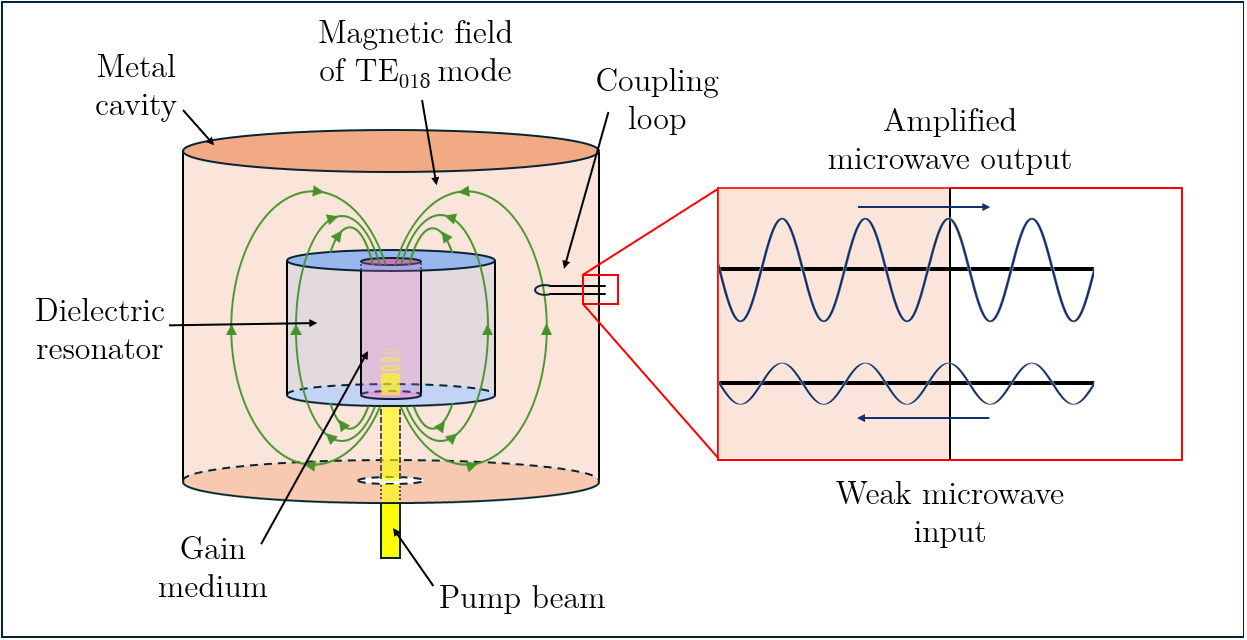
\includegraphics[width=0.8\textwidth]{figures/figure1.png}
  \caption{
    The typical anatomy of a room temperature room, with all major features
    labelled. An RF field is induced, the amplified microwave signal is output
    via the coupling.
  }
  \label{fig:figure1}
\end{figure}

The generation of a coherent microwave output (masing) relies on the transition
of atoms and molecules in the gain medium between its discrete energy levels.
When a microwave interacts with this medium, it results in the emission of
additional photons with the same frequency, phase and direction. This phenomenon
is called stimulated
emission\autocite{siegman1971introduction, purcell1995spontaneous}. Stimulated
emission occurs when an incoming photon interacts with an atom or molecule in an
excited state resulting in the emission of a second photon with identical
properties. For continual stimulated emission, there must be more atoms or
molecules in excited states than in lower states. This is called a population
inversion, shown in Figure \ref{fig:figure2}(b), and it ensures that incoming
microwaves achieve stimulated emission rather than being absorbed be the masing
crystal. A population inversion is created by supplying energy to the gain
medium (pumping), hence the need for an optical
pump\autocite{martel2000evidence}. Controlled pumping is essential for MASER
operation\autocite{oxborrow2012room,breeze2015enhanced}. A simple Jab\l{}onski
diagram in Figure \ref{fig:figure2}(a) shows the excitation of atoms using a
pump beam.

\begin{figure}[htbp]
  \centering
  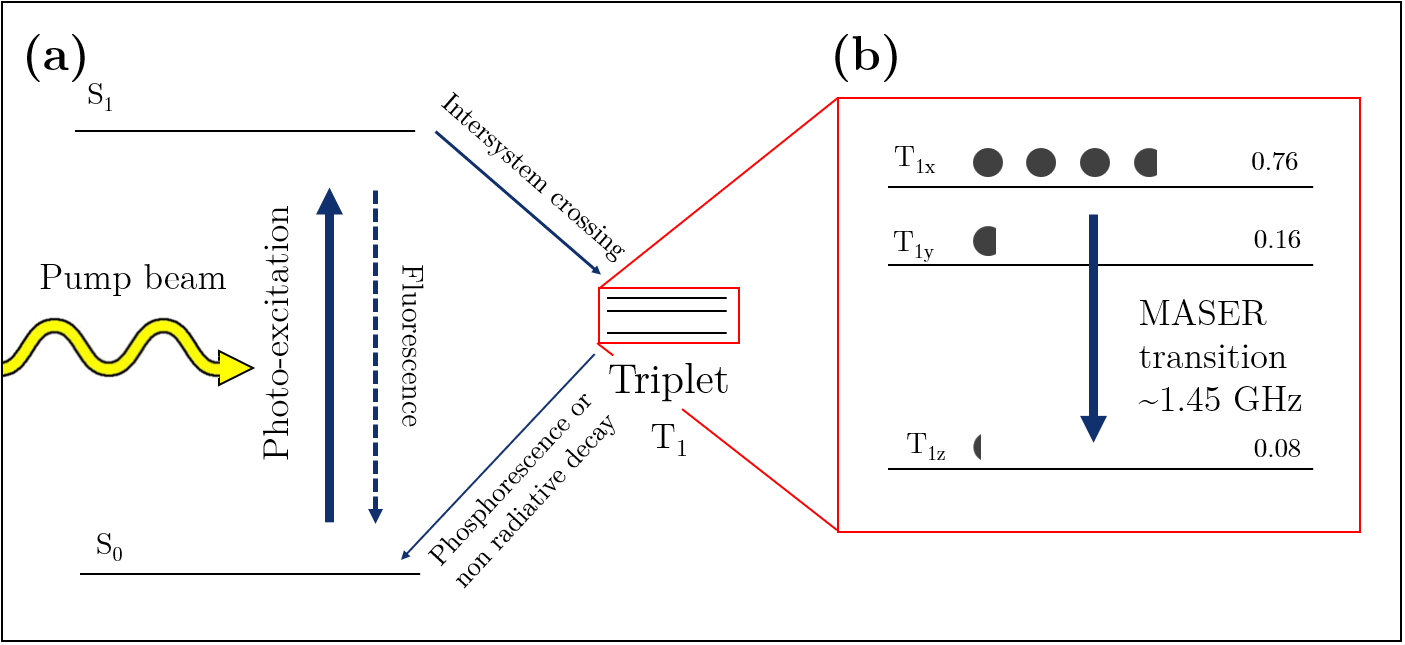
\includegraphics[width=0.8\textwidth]{figures/figure2.png}
  \caption{
    A Jab\l{}onski diagram, with (a) representing photo-excitation from the
    ground to first excited state by a pump beam and (b) the establishment of
    population inversion as $T_{1x}$ possesses $76\%$ of atoms and $T_{1z}$
    possesses only $8\%$.
  }
  \label{fig:figure2}
\end{figure}

\subsection{Role of the Microwave Cavity and Gain Medium}
\label{sec:subsection1}
Microwaves inside the metal cavity form a microwave electromagnetic field (with
the magnetic field visible in Figure \ref{fig:figure1}). The field consists of
oscillating electric and magnetic components at a frequency typically in the
gigahertz (GHz) range\autocite{griffiths2023electrodynamics}. These fields
resonate in specific spatial patterns, or cavity modes, determined by the cavity
geometry and boundary conditions. The $\text{TE}_{01\delta}$ mode is most
commonly used in MASER designs due to its high magnetic field concentration in
the dielectric region, although other modes such as the anapole mode have also
been proposed for their potential to reduce radiative losses and enhance
confinement. The electric field confinement of these modes is shown in Figure
\ref{fig:figure3}. The gain medium interacts with this electromagnetic field;
stimulated emission is driven by this
interaction\autocite{oxborrow2012room,breeze2015enhanced}. The degree to which
energy is transferred from the gain medium to photons depends on how strongly
the gain medium couples to the cavity’s
field\autocite{breeze2015enhanced, breeze2016temperature}.

\begin{figure}[htbp]
  \centering
  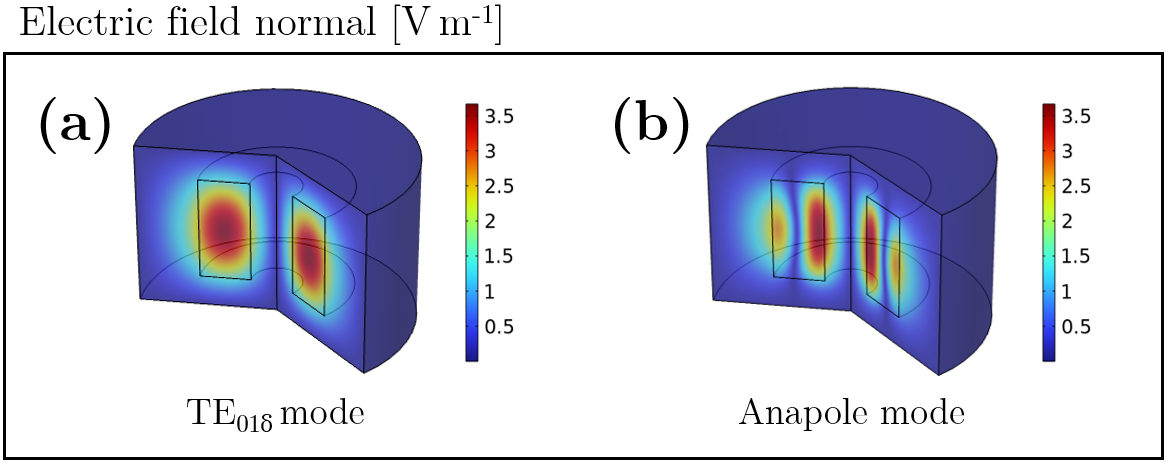
\includegraphics[width=0.9\textwidth]{figures/figure3.png}
  \caption{
    Comparison of simulated electric field normal components in COMSOL for (a)
    the $\text{TE}_{01\delta}$ mode and (b) the anapole mode. Both modes are
    shown within identical cylindrical cavities to illustrate differences in
    field distribution.
  }
  \label{fig:figure3}
\end{figure}

The system is said to enter the strong coupling regime when the rate of energy
exchange between the gain medium and the cavity photons exceeds the rate at
which energy is lost from the system. Crossing this threshold, known as the
strong coupling limit, enables the MASER to operate with higher efficiency and
greater
stability\autocite{ng2022move, breeze2015enhanced, purcell1995spontaneous}. The
strength of this interaction is quantified by the spin–photon coupling strength
g, which represents the rate of coherent energy exchange between the cavity
field and the spins in the gain medium\autocite{wen2023spin}. This coupling
strength is enhanced by increasing both the spatial overlap between the magnetic
field and the gain medium, and the density of active
spins\autocite{breeze2015enhanced,purcell1995spontaneous}. In most MASER
implementations, a coupling loop or antenna is used to extract microwave power
from the cavity or inject signals into
it\autocite{ali2020feeding, oxborrow2012room}.

\begin{equation}
  g = \frac{\mu \cdot E(r_0)}{\hbar}
    = \frac{\mu}{\hbar}
      \sqrt{\frac{\hbar \omega}{2 \varepsilon_0 \varepsilon(r_0) V_m}}
  \label{eq:coupling_rate}
\end{equation}

In this expression, $g$ is the coupling rate (Hz), $\mu$ is the transition
dipole moment of the emitter, $E(\mathbf{r}_0)$ is the electric field at the
emitter location $\mathbf{r}_0$, $\omega$ is the angular frequency of the cavity
mode, $\varepsilon_0$ is the vacuum permittivity, $\varepsilon(\mathbf{r}_0)$ is
the relative permittivity at the emitter's position, $V_{\text{m}}$ is the mode
volume, and $\hbar$ is the reduced Planck constant.


\subsection{Dielectric Resonators}
\label{sec:subsection2}
Another way to increase the number of photons produced, other than increasing
the coupling, is to increase the energy transferred into the gain medium. This
can be achieved by confining the oscillating magnetic field within the gain
medium. This is the role of the dielectric
resonator\autocite{oxborrow2012room, meher2020design}. The confinement of the
field plays a key role in determining the efficiency of energy transfer within
the device and is measured by $V_m$.

\begin{equation}
  V_{\text{m}} =
    \frac{\int \mu(\mathbf{r}) |\mathbf{H}(\mathbf{r})|^2 \, d^3\mathbf{r}}
         {\mu(\mathbf{r}_0) |\mathbf{H}(\mathbf{r}_0)|^2}
  \label{eq:mode_volume}
\end{equation}

In this expression, $\mu(\mathbf{r})$ is the permeability at position
$\mathbf{r}$, $\mathbf{H}(\mathbf{r})$ is the magnetic field distribution of the
mode, and $\mathbf{r}_0$ denotes the position of maximum magnetic energy
density.

To increase the confinement of the field (and thereby reduce $V_m$) a material
with a high relative permittivity, $\varepsilon_r$, should be used. Appendix
Table \ref{table4} shows a comparison of the most frequently used materials in
dielectric resonator design.

The dielectric resonator is therefore a crucial component in a MASER, but also
the cavity needs to be well designed to minimise system losses. Losses occur
through many mechanisms with the main types being dielectric losses (intrinsic
property of all materials,
$\tan\delta$)\autocite{krupka1998dielectric, joannopoulos2008photonic},
radiative loses (energy escaping the cavity), and conductive loses (energy
dissipated in cavity walls)\autocite{sebastian2008dielectric,chen2005analysis}.
Masing occurs when the gain provided by the inverted spin population exceeds the
total cavity losses, defining the masing threshold
condition\autocite{zollitsch2023maser}. Figure \ref{fig:figure4} shows the
difference in $V_m$ between a cavity with and without a dielectric resonator.

\begin{figure}[htbp]
  \centering
  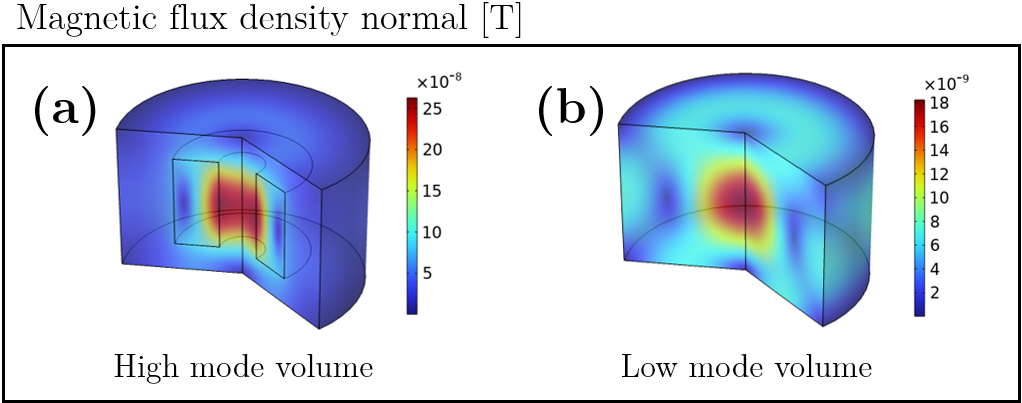
\includegraphics[width=0.9\textwidth]{figures/figure4.png}
  \caption{
    Magnetic flux density normal plots from COMSOL comparing (a) a cavity with a
    dielectric resonator, resulting in high mode volume, and (b) a cavity
    without a dielectric resonator, thus showing reduced mode volume due to a
    reduction in field confinement.
  }
  \label{fig:figure4}
\end{figure}

\section{Recent Developments}
\label{sec:section2}
The first successful operation of a room-temperature solid-state MASER in 2012
marked a significant breakthrough in the field. This device utilised a
pentacene-doped p-terphenyl crystal as the gain medium, optically pumped by a
pulsed dye laser emitting at 590 nm\autocite{oxborrow2012room}. The system
achieved stimulated emission at approximately 1.45 GHz without the need for
cryogenic cooling or external magnetic fields. The pentacene molecules, upon
optical excitation, underwent intersystem crossing to a triplet state, leading
to a population inversion essential for
masing\autocite{salvadori2017nanosecond,oxborrow2012room}.

Despite this advancement, the initial design faced challenges. The MASER
operated only in pulsed mode, with high optical pumping power requirements
($\sim$ 1.4 kW), and suffered from significant dielectric and radiative losses
within the cavity, limiting its efficiency and practical
applications\autocite{
  salvadori2017nanosecond,arroo2021perspective,breeze2015enhanced
}.

Subsequent research focused on improving dielectric resonator designs to enhance
MASER performance. High-permittivity materials such as strontium titanate
(\ce{SrTiO3}) and titanium dioxide (\ce{TiO2}) were explored to reduce mode
volume and increase the Purcell factor, thereby strengthening the coupling
between the cavity field and the gain
medium\autocite{howard1991rutile, goryachev2015sto, rupprecht1962sto}.
Innovations in resonator geometries, including the use of whispering-gallery
modes and photonic crystal structures, have been investigated to achieve higher
quality factors and better field confinement
\autocite{
  rybin2017high, campione2016broken, oxborrow2007traceable, krupka1999whispering
}.

Efforts to identify alternative gain media led to the exploration of
diazapentacene-doped p-terphenyl, which demonstrated improved chemical stability
and lower masing thresholds compared to pentacene-based systems. Additionally,
nitrogen-vacancy (NV) centers in diamond have been proposed as potential
room-temperature gain media due to their long spin coherence times and
compatibility with continuous-wave
operation\autocite{
  breeze2018continuous,sherman2022diamond,sherman2021performance,jin2015proposal
}.

Recent developments have aimed at miniaturizing MASER systems for practical
applications. The "MASER-in-a-Shoebox" project successfully demonstrated a
portable, plug-and-play MASER device operating at room temperature and zero
magnetic field, highlighting the potential for MASER technology in real-world
scenarios\autocite{ng2023maser}.

Other research has explored various dielectric resonator geometries to enhance
MASER performance. Traditional cylindrical and rectangular shapes have been
complemented by innovative designs such as hemispherical, hexagonal, conical,
and trapezoidal forms\autocite{meher2020design}. These geometries aim to
optimise field confinement and mode distribution, thereby improving the
resonator's quality factor and reducing mode
volume\autocite{rybin2017high, campione2016broken}. For instance, asymmetric
cross-shaped dielectric resonators have demonstrated wideband circular
polarisation, which can be beneficial in certain MASER applications.

\section{The Purcell Factor}
\label{sec:section3}
Dielectric resonators serve a critical function in MASERs by concentrating the
magnetic flux within the gain medium, thereby enhancing the interaction between
the electromagnetic field and the active material. This concentration is pivotal
for achieving the strong coupling regime necessary for efficient MASER
operation\autocite{oxborrow2012room, ng2022move}. The geometry and material
properties of the resonator directly influence the distribution and intensity of
the electromagnetic fields, affecting the device's overall
performance\autocite{rybin2017high}. The performance of a dielectric resonator
in a MASER is fundamentally determined by two interrelated metrics: the quality
factor ($Q_f$) and $V_m$. The quality factor measures how long energy is stored
in the resonator before it is lost, whether through dielectric absorption or any
other losses in the system\autocite{green1955story}. A high $Q_f$ value implies
low intrinsic loss, enabling the resonator to sustain strong electromagnetic
fields over longer periods. Figure \ref{fig:figure5} demonstrates the
dissipation of energy with time in a high and low quality factor resonator. This
sustained field is critical for facilitating multiple interactions between the
gain medium and the cavity field, which increases the probability of stimulated
emission\autocite{lefloch2008bragg}. The mode volume has already been defined
and can be seen in Eq \ref{eq:mode_volume}.

\begin{figure}[htbp]
  \centering
  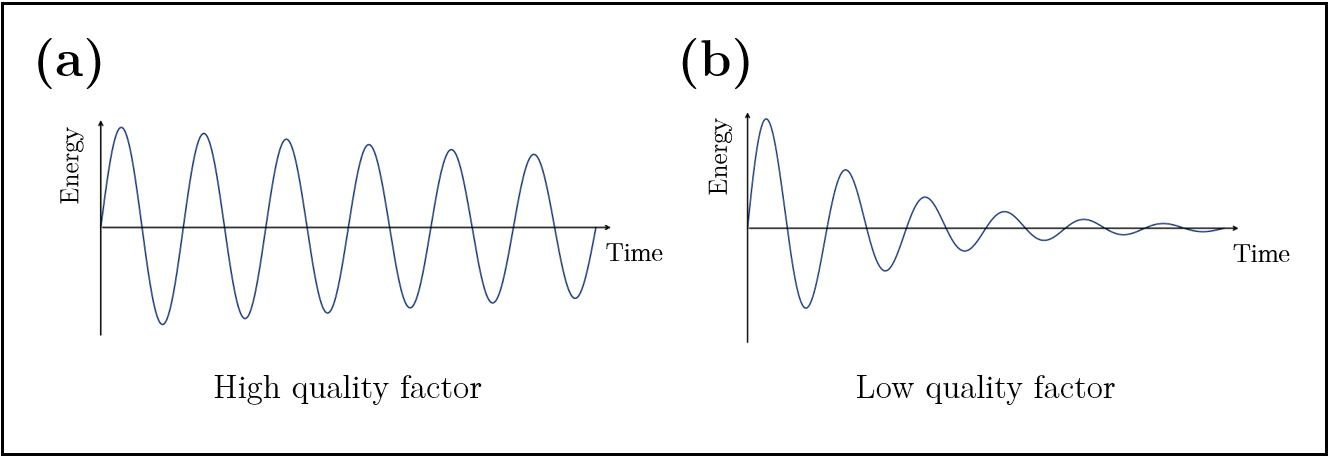
\includegraphics[width=0.9\textwidth]{figures/figure5.png}
  \caption{
    Graphical comparison of (a) high quality factor and (b) low quality factor
    resonators, showing how energy decays over time. High-Q systems retain
    energy longer with slower decay, while low-Q systems dissipate energy
    rapidly.
  }
  \label{fig:figure5}
\end{figure}

These two parameters combine to define the Purcell factor ($F_p$), a measure of
how much the cavity enhances the spontaneous emission rate of the gain medium.
The Purcell factor is given by:

\begin{equation}
  \mathbf{F}_{\text{P}} =
    \frac{3}{4\pi^2}
    \left(\frac{\lambda_{\text{free}}}{n}\right)^3
    \frac{Q}{V_m}
  \label{Purcell}
\end{equation}

where $\lambda_{\text{free}}$ is the free-space wavelength of the emitter, and
$n$ is the refractive index of the medium.

In the context of MASERs, a high Purcell factor implies enhanced emission and
increased likelihood of reaching the masing threshold, especially in systems
with limited pump power or low intrinsic gain.

Recent studies have demonstrated that by carefully tailoring dielectric
resonator geometries, such as incorporating notches, split-rings, or using
hybrid photonic structures, both $Q_f$ and $V_m$ can be optimised
simultaneously\autocite{campione2016broken}. For example, Rybin et al. showed
that supercavity modes in subwavelength dielectric resonators can yield
ultra-high $Q$ factors by exploiting interference between leaky and non-leaky
modes to trap energy more effectively\autocite{rybin2017high}. Similarly,
broken-symmetry designs have been used to excite Fano resonances, leading to
sharp spectral features with high $Q_f$ and relatively small $V_m$, offering a
practical route to maximise the Purcell enhancement in compact
geometries\autocite{campione2016broken}.

A key related parameter is the cooperativity, $C$, which quantifies the ratio of
coherent coupling to dissipation in the
system\autocite{wen2023spin,sherman2021performance}. It is often expressed as:

\begin{equation}
  C = \frac{g^2}{\kappa \gamma}
\end{equation}

where $g$ is the spin–photon coupling strength, $\kappa$ is the cavity decay
rate, and $\gamma$ is the spin dephasing rate.

Since a high Purcell factor enhances the interaction strength between the cavity
field and the gain medium, it directly contributes to increasing cooperativity.
High cooperativity is essential for efficient masing and is closely associated
with low noise output, making it a critical for practical MASER applications in
sensing and communication systems\autocite{sherman2021performance}.

\section{COMSOL Modelling of Resonators}
\label{sec:section4}
In the design and optimisation of MASERs, a software is required that can
accurately model the electromagnetic fields within dielectric resonators. COMSOL
Multiphysics\textregistered{}, a finite element analysis software, is widely
utilised for this purpose due to its capability to simulate complex geometries
and material properties\autocite{comsol2020intro,comsol2020rf,comsol2024doc}. By
solving Maxwell's equations, COMSOL enables the visualisation and analysis of
electric $\vec{\mathbf{E}}$ and magnetic $\vec{\mathbf{H}}$ field distributions
within resonators. This is essential for determining the $Q_f$ and
$V_m$\autocite{zienkiewicz2013errors,}. In COMSOL, Q can be calculated by
integrating the electromagnetic energy density over the resonator volume and the
power loss over its surface[48,50]. This approach has been demonstrated in
COMSOL's application examples, where models of rectangular, cylindrical, and
spherical cavities are analysed to compute resonant frequencies and
$Q_f$\autocite{comsol2024doc}. Additionally, COMSOL's eigenfrequency analysis
allows for the determination of resonant modes and their corresponding field
distributions, allowing for the identification of modes with optimal $Q_f$/$V_m$
ratios.

\begin{equation}
  Q_f = \frac{1}{\tan \delta}=\frac{\varepsilon'}{\varepsilon''}
  \label{eq:Q}
\end{equation}

Where $Q_f$ is the quality factor due to dielectric losses, $\tan\delta$ is the
loss tangent of the material defined as $\tan\delta$, $\varepsilon'$ is the real
part of the complex permittivity, and $\varepsilon''$ is the imaginary part
(loss component) of the complex permittivity.

$V_m$ quantifies the spatial confinement of the resonant mode and is calculated
by integrating the energy density over the entire volume and normalizing it to
the maximum energy density within the resonator. COMSOL's capability to model
complex resonator geometries, including whispering-gallery modes and photonic
crystal structures, enables the exploration of designs that achieve high
Q-factors and low mode volumes.

Additionally, COMSOL has been employed in the simulation of circuit quantum
electrodynamics (cQED) systems, where superconducting qubits interact with
microwave resonators. In these applications, precise modelling of
$\vec{\mathbf{E}}$ and $\vec{\mathbf{H}}$ fields is essential for understanding
light-matter interactions at the quantum level and for designing resonators with
desired coupling strengths and coherence times\autocite{oxborrow2007traceable}.

\section{Gaps in Current Literature and Motivation for This Project}
\label{sec:section5}
Despite extensive progress in MASER development, there remains a notable gap in
the literature regarding the systematic optimisation of dielectric resonator
shapes and sizes. While several studies have investigated material properties
and mode confinement within standard geometries such as cylindrical or spherical
resonators\autocite{meher2020design}, none have explored beyond these
conventional designs to determine how variations in shape could influence the
quality factor, mode volume, and, by extension, the Purcell factor. Although
simulation tools such as COMSOL Multiphysics\textregistered{} have been employed
to model specific dielectric resonators in MASER and photonic systems, the
parameter space of resonator geometry itself remains largely unexplored in terms
of global optimisation\autocite{karpov2022evolutionary,stanovov2022automatic}.

To address this gap, the present project focuses on optimising the size and
shape of dielectric resonators using the COMSOL API in conjunction with a
genetic algorithm (GA). The goal is to maximise the Purcell factor by enhancing
electromagnetic confinement and improving $Q_f$/$V_m$[13,21]. This approach
allows for automated exploration of complex geometric configurations that may
not be intuitive or easily accessible through manual
tuning\autocite{goh2006design,karpov2022evolutionary,stanovov2022automatic}. By
treating the resonator geometry as a set of evolutionary parameters within the
GA, the simulation framework identifies structures that yield superior field
confinement and reduced radiative and dielectric
losses\autocite{tsuji2009multi,monzo2007application}. Beyond the scope of this
project, future work could investigate integrating machine learning models to
predict resonator performance or applying this methodology to other active
materials and frequency bands could further extend the impact of this
optimisation framework within both MASER and broader photonic technologies.
While this study focuses on simulation-based optimisation, future work could
also include experimental fabrication and testing of high-Purcell resonator
designs to validate model predictions\autocite{ng2022move,ng2023maser}.

\section{Summary}
\label{sec:section6}
MASERs (Microwave Amplification by Stimulated Emission of Radiation) operate on
the same fundamental principle as lasers but emit coherent radiation in the
microwave regime. Initially constrained by the need for cryogenic environments
and external magnetic fields, a major milestone was achieved in 2012 with the
demonstration of a room-temperature MASER using pentacene-doped p-terphenyl as
the gain medium within a dielectric-loaded cavity. This system emitted at 1.45
GHz, but despite its breakthrough status, it remained limited to pulsed
operation and suffered from high optical pump power demands and significant
losses due to cavity radiation and dielectric absorption.

Recent developments have focused on improving MASER efficiency and stability by
enhancing the electromagnetic confinement offered by dielectric resonators.
Innovations in resonator geometries, including non-standard shapes and photonic
crystal structures, aim to improve the cavity’s quality factor ($Q_f$) while
reducing mode volume ($V_m$), thereby increasing the Purcell factor
(proportional to $Q_f$/$V_m$), a critical measure of the system's emission
enhancement. High-permittivity, low-loss materials such as \ce{SrTiO3} and
\ce{TiO2} are commonly investigated to further improve performance. However,
most studies to date have relied on conventional resonator geometries, with
little attention paid to shape optimisation.

This project addresses that gap by using COMSOL Multiphysics\textregistered{} in
combination with a genetic algorithm to automatically optimise the size and
shape of dielectric resonators for maximum Purcell factor. By simulating the
magnetic field distributions and calculating $Q_f$ and $V_m$, the algorithm
searches for configurations that offer superior field confinement and reduced
energy loss. The approach aims to identify unconventional resonator shapes that
may provide substantial performance gains. Future work could extend this
methodology through machine learning models, offering new directions in both
MASER and photonic device design.
